\section{Sharding}

El objetivo de esta sección es analizar la distribución de la carga en una colección repartida entre varios shards.

La estructura de los documentos es la siguiente:

\begin{listing}
\begin{minted}[frame=single,
               framesep=3mm,
               linenos=true,
               xleftmargin=21pt,
               tabsize=4]{js}
{
  "nombre": nombrePersona
  "password": passwordPersona
  "codigo_postal": getRandomIntInclusive(1, 1000000),
  "genero": generoPersona,
  "edad": edadPersona
  "fecha_creacion": fechaCreacion
}

\end{minted}
\caption{Ejemplo persona}
\label{json-example}
\end{listing}

La shard key se establece a partir del atributo \emph{codigo\_postal}, generado de forma pseudoaleatoria.
Los documentos son agregados en bloques de 20.000 documentos, hasta alcanzar un total de 500.000. El tamaño
total de la colección es aproximadamente 115 MB. Esto genera un total de 25 mediciones por experimento.

Es posible generar los shards de 2 formas posibles sobre la shard key:
\begin{itemize}
\item Por rango
\item Por hash
\end{itemize}

Por cada uno de estos tipos realizamos un experimento con 2 y 3 shards.

\subsection{Partición basada en rango}

\begin{figure}[!h]
  \begin{center}
      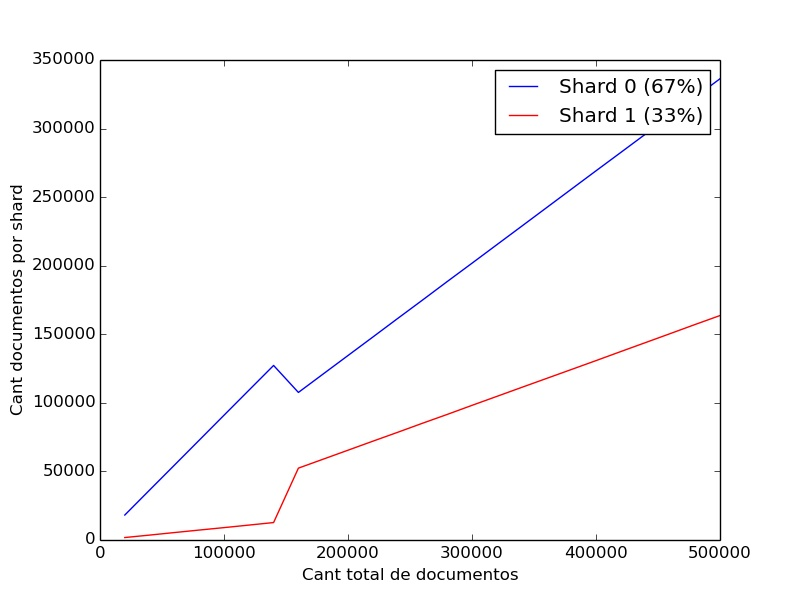
\includegraphics[scale=0.4]{imagenes/range1.jpg}
      \caption{2 Shards utilizando partición de keys por rango}
      \label{fig:contra1}
  \end{center}
\end{figure}

~

La carga no se reparte uniformemente. El shard 0 mantiene un aproximadamente un 67\% de los datos a lo largo de todo
el experimento, mientras que el segundo shard mantiene el 33\% de los datos.

\begin{figure}[!h]
  \begin{center}
      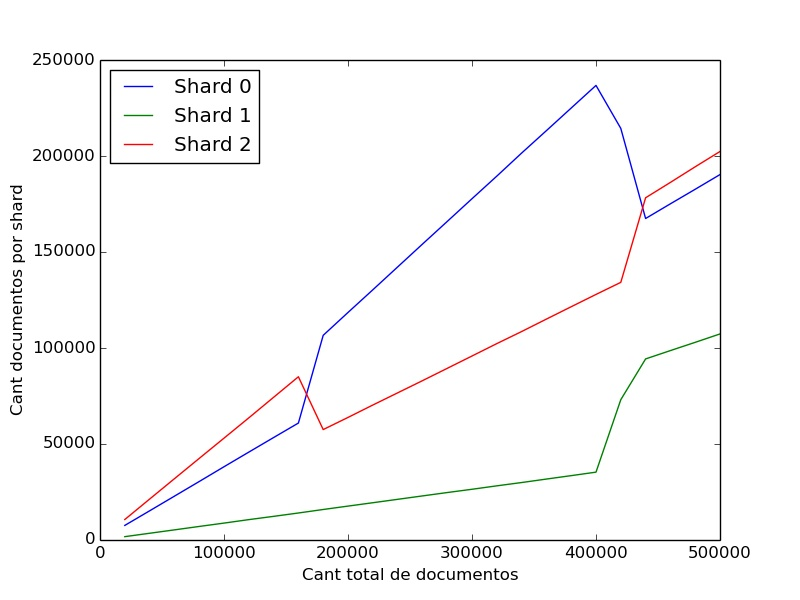
\includegraphics[scale=0.4]{imagenes/range2.jpg}
      \caption{3 Shards utilizando partición de keys por rango}
      \label{fig:contra1}
  \end{center}
\end{figure}

~

La existencia de un tercer shard favorece al balance de la carga, aunque sigue habiendo un shard que contiene
pocos datos.

\subsection{Partición basada en hash}

\begin{figure}[!h]
  \begin{center}
      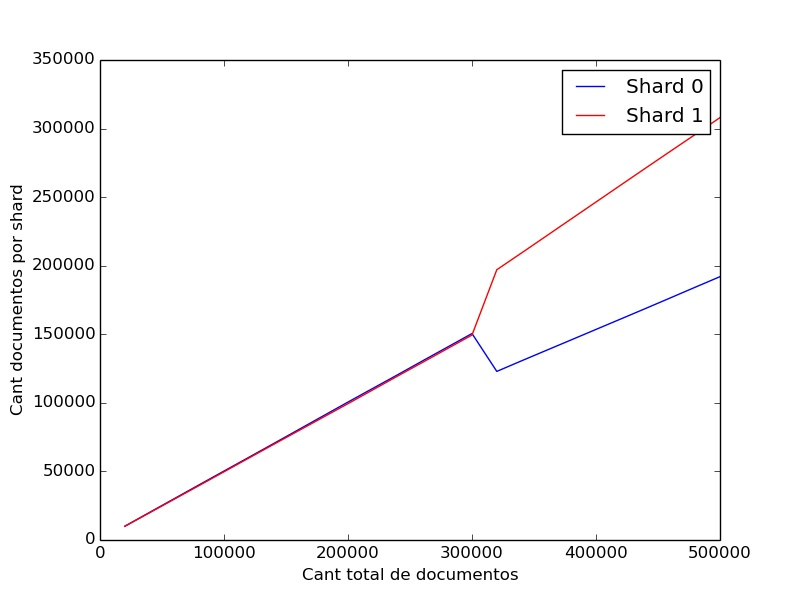
\includegraphics[scale=0.4]{imagenes/hash1.jpg}
      \caption{2 Shards utilizando partición de keys basada en hash}
      \label{fig:contra1}
  \end{center}
\end{figure}

~

La carga se distribuye de manera uniforme hasta un punto de quiebre, en donde un shard queda con más carga que
el otro.

\begin{figure}[!h]
  \begin{center}
      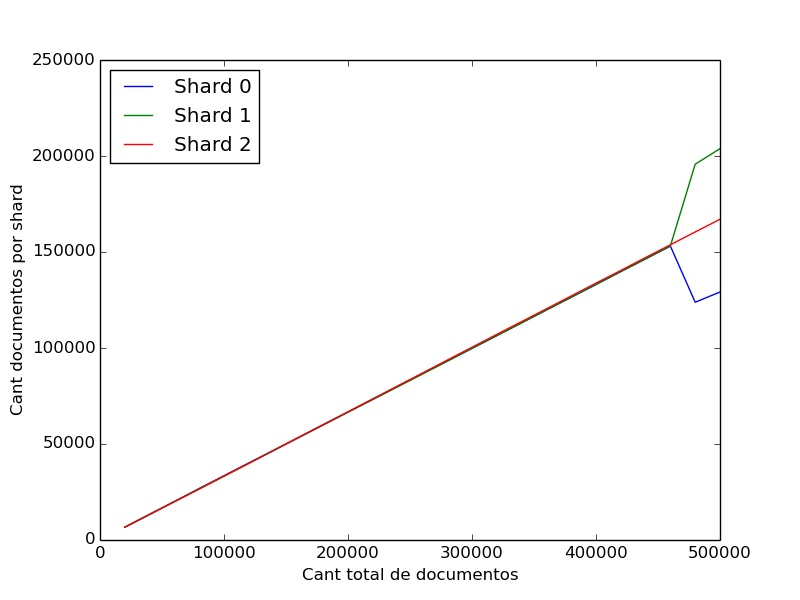
\includegraphics[scale=0.4]{imagenes/hash2.jpg}
      \caption{3 Shards utilizando partición de keys basada en hash}
      \label{fig:contra1}
  \end{center}
\end{figure}

~

Nuevamente, la existencia de un tercer shard aporta estabilidad al balanceo. En este caso, la distribución
se mantiene uniforme casi hasta el final de la experimentación. En dicho punto, los shards quedan
con una distribución levemente diferente.

~

\subsection{Conclusión}

Para valores de shard keys generados de forma pseudoaleatoria es conveniente tener una clustering key
basada en hash para mantener el balanceo uniforme por sobre una con rango.
La existencia de mayor cantidad de shards favorecen a la uniformidad de la distribución.

